% bei Standalone in documentclass noch:
% \RequirePackage{luatex85}

\documentclass[captions=tableheading, titlepage= firstiscover, parskip = half , bibliography=totoc]{scrartcl}
%paper = a5 fÃŒr andere optinen
% titlepage= firstiscover
% bibliography=totoc fÃŒr bibdateien
% parskip=half  VerÀnderung um AbsÀtze zu verbessern

\usepackage{scrhack} % nach \documentclass
\usepackage[aux]{rerunfilecheck}
\usepackage{polyglossia}
\usepackage[style=numeric, backend=biber]{biblatex} % mit [style = alphabetic oder numeric] nach polyglossia
\addbibresource{lit.bib}
\setmainlanguage{german}

\usepackage[autostyle]{csquotes}
\usepackage{amsmath} % unverzichtbare Mathe-Befehle
\usepackage{amssymb} % viele Mathe-Symbole
\usepackage{mathtools} % Erweiterungen fÃŒr amsmath
\usepackage{fontspec} % nach amssymb
% muss ins document: \usefonttheme{professionalfonts} % fÌr Beamer PrÀsentationen
\usepackage{longtable}
\usepackage{dsfont}
\usepackage[
math-style=ISO,    % \
bold-style=ISO,    % |
sans-style=italic, % | ISO-Standard folgen
nabla=upright,     % |
partial=upright,   % /
]{unicode-math} % "Does exactly what it says on the tin."
\setmathfont{Latin Modern Math}
% \setmathfont{Tex Gyre Pagella Math} % alternativ

\usepackage[
% die folgenden 3 nur einschalten bei documenten
locale=DE,
separate-uncertainty=true, % Immer Fehler mit ±
per-mode=symbol-or-fraction, % m/s im Text, sonst \frac
]{siunitx}

% alternativ:
% per-mode=reciprocal, % m s^{-1}
% output-decimal-marker=., % . statt , fÃŒr Dezimalzahlen

\usepackage[
version=4,
math-greek=default,
text-greek=default,
]{mhchem}

\usepackage[section, below]{placeins}
\usepackage{caption} % Captions schöner machen
\usepackage{graphicx}
\usepackage{grffile}
\usepackage{subcaption}

% \usepackage{showframe} Wenn man die Ramen sehen will

\usepackage{float}
\floatplacement{figure}{htbp}
\floatplacement{table}{htbp}

\usepackage{mathtools}

\usepackage{booktabs}

 \usepackage{microtype}
 \usepackage{xfrac}

 \usepackage{expl3}
 \usepackage{xparse}

 % \ExplSyntaxOn
 % \NewDocumentComman \I {}  %Befehl\I definieren, keine Argumente
 % {
 %    \symup{i}              %Ergebnis von \I
 % }
 % \ExplSyntaxOff

 \usepackage{pdflscape}
 \usepackage{mleftright}

 % Mit dem mathtools-Befehl \DeclarePairedDelimiter können Befehle erzeugen werden,
 % die Symbole um AusdrÃŒcke setzen.
 % \DeclarePairedDelimiter{\abs}{\lvert}{\rvert}
 % \DeclarePairedDelimiter{\norm}{\lVert}{\rVert}
 % in Mathe:
 %\abs{x} \abs*{\frac{1}{x}}
 %\norm{\symbf{y}}

 % FÃŒr Physik IV und Quantenmechanik
 \DeclarePairedDelimiter{\bra}{\langle}{\rvert}
 \DeclarePairedDelimiter{\ket}{\lvert}{\rangle}
 % <name> <#arguments> <left> <right> <body>
 \DeclarePairedDelimiterX{\braket}[2]{\langle}{\rangle}{
 #1 \delimsize| #2
 }

\setlength{\delimitershortfall}{-1sp}

 \usepackage{tikz}
 \usepackage{tikz-feynman}

 \usepackage{csvsimple}
 % Tabellen mit \csvautobooktabular{"file"}
 % muss in table umgebung gesetzt werden


% \multicolumn{#Spalten}{Ausrichtung}{Inhalt}

\usepackage{hyperref}
\usepackage{bookmark}
\usepackage[shortcuts]{extdash} %nach hyperref, bookmark

\newcommand{\ua}[1]{_\symup{#1}}
\newcommand{\su}[1]{\symup{#1}}

\begin{document}
\section{Zielsetzung}
Ziel dieses Versuchs ist es die Streuung von $\su{\alpha}$-Teilchen an einer Goldfolie zu bestimmen.
Dafür wird der differentielle Wirkungsquerschnitt der Streuung und die Abhängigkeit der Kernladungszahl Z
des Targetmaterials untersucht. \newline
Aus der Streuung kann zusätzlich durch die Energieverlustmessung der $\su{\alpha}$-Teilchen
auch die Foliendicke bestimmt werden.
\section{Theorie}
Beim Durchlauf von positiv geladenen $\su{\alpha}$-Teilchen durch Materie kann es zu
zwei unterschiedlichen Wechselwirkungen kommen. Die erste Wechselwirkung findet mit negativ geladenen Hüllenelektron
statt und die zweite mit dem positiven Atomkern.
\newline
Bei der Wechselwirkung zwischen $\su{\alpha}$-Teilchen und dem Hüllenelektronen kommt es durch
Anregungs- und Ionisationsprozesse zur Energieabgabe.
Es wird angenommen, dass es aufgrund der größeren Masse der $\su{\alpha}$-Teilchen gegenüber
der Elektronenmasse zu keiner Ablenkung der $\su{\alpha}$-Teilchen kommt.
\newline
Die Bethe-Bloch-Gleichung beschreibt den Energieverlust
\begin{equation*}
    -\frac{dE}{dx} = -\frac{4\pi e^4z^2NZ}{m_0v^2(4\pi \epsilon_0)^2} \ln \frac{2m_0v^2}{I}
\label{eqn:bethebloch}
\end{equation*}
der $\su{\alpha}$-Teilchen beim Durchgang durch die Materie.
Hierbei gibt N die Atomdichte, $\su{m_0}$ die Ruheenergie des Hüllenelektrons, Z die Kernladungszahl und I die mittlere Ionisationsenergie
des Targetmaterials an.

Bei der Streuung der $\su{\alpha}$-Teilchen am Atomkern kommt es durch die Coulombkraft zu
einer Richtungsänderung um den Streuwinkel $\su{\Theta}$. Es wird nach der 1. Born'schen Näherung davon
ausgegangen, dass die Mehrfachstreuung der $\su{\alpha}$-Teilchen vernachlässigt werden kann.
\newline
Dieser Streuwinkel lässt sich mit der Rutherford-Streuformel berechnen
\begin{equation*}
    \frac{d\sigma}{d\Omega}(\Uptheta) = \frac{1}{(4\pi \epsilon_0)^2} \Big(\frac{zZe^2}{4E_{\alpha}}\Big)^2 \frac{1}{\sin^4\frac{\Uptheta}{2}}.
\end{equation*}
$\su{E_{\alpha}}$ beschreibt dabei die mittlere kinetische Enegie der $\su{\alpha}$-Teilchen .
Der differentielle Wirkungsquerschnitt $\frac{d\sigma}{d\Omega}$ beschreibt gerade die Intensitätsverteilung
der gestreuten $\su{\alpha}$-Teilchen in den Raumwinkel $\su{\Uptheta}$.

\newpage
\section{Versuchsaufbau}
Der Versuchsaufbau ist in Abbildung \ref{fig:aufbau} dargestellt.
\begin{figure}
  \centering
  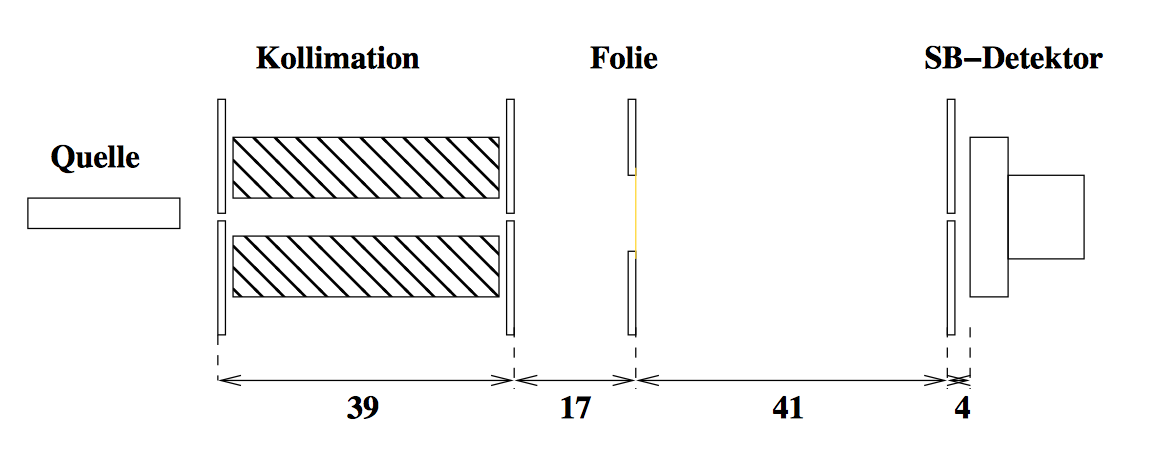
\includegraphics[width = 12 cm]{pictures/aufbau.png}
  \caption{Darstellung des Versuchsaufbaus}
  \label{fig:aufbau}
\end{figure}
\newline
Der Versuch findet im Vakuum statt, da die $\su{\alpha}$-Strahlung in Luft nur eine sehr geringe
Reichweite hat. Als $\su{\alpha}$-Strahler dient ein $\ce{^{241}}\su{Am}$-Präparat.
Die aus der Quelle austretenen Teilchen werden mithilfe von zwei 2\,mm Schlitzblenden kollimiert,
damit diese senktrecht auf die Goldfolie treffen.
An dieser Folie werden die Teilchen um den Winkel $\su{\Uptheta}$ gestreut und von einem Detektor
aufgenommen. Bei diesem Detektor handelt es sich um einen Surface-Barrier-Detektor, also einen
Halbleiter Detektor, an dem die einfallenden $\su{\alpha}$-Teilchen in der Sperrschicht Elektronen-Loch-Paare
erzeugen und durch ihre Energieabgabe die Exzitonen in ein höheres Energieniveau anheben, wo diese frei beweglich sind.
Durch ein anliegendes elektrisches Feld werden diese zur jeweiligen Elektorde beschleunigt.
Die führt zu einem messbaren Stromimpuls an den Elektroden. Um die vom Detektor erfassten Impulse besser verarbeiten
zu können, wird ein Verstärker verwendet.
Als Messgeräte dienen dann ein Oszilloskop zur Bestimmung des Energieverlusts und ein Zählwerk zur
Bestimmung des Streuquerschnitts.

\section{Durchführung}
Zu Beginn des Versuches wird die Apparatur über eine Vakuumspumpe evakuiert.
Um einen geraden Durchtritt der $\su{\alpha}$-Teilchen zu gewährleisten, wird der Detektor justiert.
\newline
Für die Bestimmung der Foliendicke wird eine Energieverlustmessung durchgeführt.
Dabei werden die Pulshöhen der Detektorpulse in Abhängigkeit des Kammerdrucks aufgenommen.
Durch das Feindrosselventil kann der Kammerdruck langsam erhöht werden.
Zur Ermittlung der mittleren Pulshöhe wird das Oszilloskop in das Programm "Nachleuchten" gestellt,
an dem dann die Pulshöhen abgelesen werden können.\newline
Diese Messung wird einmal mit und einmal ohne Goldfolie durchgeführt..
\newline
Um den differentiellen Wirkungsquerschnitt einer Goldfolie zu bestimmen, wird die Zählrate in Abhängigkeit
des Streuwinkels $\su{\Uptheta}$ aufgenommen. Dafür werden unterschiedliche Winkel eingestellt.
Die Dauer der Messung wird durch den statistischen Fehler der Zählrate
$\sqrt{I}$ festgelegt, da der $\su{\alpha}$-Zerfall poissonverteilt ist.
\newline
Zur Untersuchung der Mehrfachstreuung wird die Streuung der unterschiedliche Folien gemessen. Dafür wird ein fester Winkel
eingestellt.
\newline
Die Aktivität wird außerdem ohne Folie für 120\,s im Vakuum gemessen.
\end{document}
